\chapter{Variables and types}
\label{chap02}

\section{More printing}
\index{print}
\index{statement!print}

You can put as many
statements as you want in {\tt main}; for example, to
print more than one line:

\begin{lstlisting}
class Hello {

  // Generates some simple output.

  public static void main(String[] args) {
    System.out.println("Hello, world.");     // print one line
    System.out.println("How are you?");      // print another
  }
}
\end{lstlisting}
%
As this example demonstrates, you can put comments at the
end of a line, as well as on a line by themselves.

\index{String}
\index{type!String}

The phrases that appear in quotation marks are called {\bf strings},
because they are made up of a sequence (string) of characters.
Strings can contain any combination of letters, numbers, punctuation
marks, and other special characters.

\index{newline}

{\tt println} is short for ``print line,'' because after each
line it adds a special character, called a {\bf newline}, that
moves the cursor to the next line of the display.
The next time {\tt println} is invoked, the new text appears
on the next line.

To display the output from multiple print
statements all on one line, use {\tt print}:

\begin{lstlisting}
class Hello {

  // Generates some simple output.

  public static void main(String[] args) {
    System.out.print("Goodbye, ");
    System.out.println("cruel world!");
  }
}
\end{lstlisting}
%
The output appears on a single line as
{\tt Goodbye, cruel world!}.  There is a space
between the word ``Goodbye'' and the second quotation mark.
This space appears in the output, so it affects the behavior
of the program.

Spaces that appear outside of quotation marks generally do
not affect the behavior of the program.  For example, I
could have written:

\begin{lstlisting}
class Hello {
public static void main(String[] args) {
System.out.print("Goodbye, ");
System.out.println("cruel world!");
}
}
\end{lstlisting}
%
This program would compile and run just as well as the original.
The breaks at the ends of lines (newlines) do not affect
the program's behavior either, so I could have written:

\begin{lstlisting}
class Hello { public static void main(String[] args) {
System.out.print("Goodbye, "); System.out.println
("cruel world!");}}
\end{lstlisting}
%
That would work, too, but
the program is getting harder and harder to read.  Newlines and
spaces are useful for organizing your program visually, making
it easier to read the program and locate errors.


\section {Variables}
\index{variable}
\index{value}

One of the most powerful features of a programming language is the
ability to manipulate {\bf variables}.  A variable is a named location
that stores a {\bf value}.  Values are things that can be printed, stored
and (as we'll see later) operated on.  The strings we have been
printing ({\tt "Hello, World."}, {\tt "Goodbye, "}, etc.)  are values.

To store a value, you have to create a variable.  Since
the values we want to store are strings, we declare that
the new variable is a string:

\begin{lstlisting}
    String bob;
\end{lstlisting}
%
This statement is a {\bf declaration}, because it declares that the
variable named {\tt bob} has the type {\tt String}.  Each variable
has a type that determines what kind of values it can store.  For
example, the {\tt int} type can store integers, and the {\tt String}
type can store strings.

\index{declaration}
\index{statement!declaration}

Some types begin with a capital letter and some
with lower-case.  We will learn the significance of this distinction
later, but for now you should take care to get it right.  There is no
such type as {\tt Int} or {\tt string}, and the compiler will object
if you try to make one up.

To create an integer variable, the syntax is {\tt int bob;},
where {\tt bob} is the arbitrary name you made up for the
variable.  In general, you will want to make up variable names
that indicate what you plan to do with the variable.  For
example, if you saw these variable declarations:

\begin{lstlisting}
    String firstName;
    String lastName;
    int hour, minute;
\end{lstlisting}
%
you could guess what values
would be stored in them.  This example
also demonstrates the syntax for declaring multiple variables
with the same type: {\tt hour} and {\tt second}
are both integers ({\tt int} type).

\section{Assignment}
\index{assignment}
\index{statement!assignment}

Now that we have created variables, we want to
store values.  We do that with an {\bf assignment
statement}.

\begin{lstlisting}
    bob = "Hello.";      // give bob the value "Hello."
    hour = 11;           // assign the value 11 to hour
    minute = 59;         // set minute to 59
\end{lstlisting}
%
This example shows three assignments, and the comments show
three different ways people sometimes talk about assignment
statements.  The vocabulary can be confusing here, but the
idea is straightforward:

\begin{itemize}

\item When you declare a variable, you create a named storage location.

\item When you make an assignment to a variable, you give it a value.

\end{itemize}

A common way to represent variables on paper is to draw a box
with the name of the variable on the outside and the value
of the variable on the inside.  This figure shows
the effect of the three assignment statements:


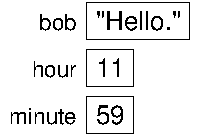
\includegraphics{figs/assign.pdf}


As a general rule,
a variable has to have the same type as the
value you assign it.  You cannot store a {\tt String} in {\tt minute} or an
integer in {\tt bob}.

On the other hand, that rule can be confusing, because there are many
ways that you can convert values from one type to another, and Java
sometimes converts things automatically.  For now you should
remember the general rule, and we'll talk about exceptions later.

Another source of confusion is that some strings {\em look}
like integers, but they are not.  For example, {\tt bob}
can contain the string {\tt "123"}, which is made up of the
characters {\tt 1}, {\tt 2} and {\tt 3}, but that is not
the same thing as the {\em number} {\tt 123}.

\begin{lstlisting}
    bob = "123";     // legal
    bob = 123;       // not legal
\end{lstlisting}


\section{Printing variables}
\label{printing}

You can print the value of a variable using {\tt println} or
{\tt print}:

\begin{lstlisting}
class Hello {
  public static void main(String[] args) {
    String firstLine;
    firstLine = "Hello, again!";
    System.out.println(firstLine);
  }
}
\end{lstlisting}
%
This program creates a variable named {\tt firstLine}, assigns
it the value {\tt "Hello, again!"} and then prints that value.
When we talk about ``printing a variable,'' we mean printing
the {\em value} of the variable.  To print the {\em name} of
a variable, you have to put it in quotes.
For example: {\tt System.out.println("firstLine");}

For example, you can write

\begin{lstlisting}
    String firstLine;
    firstLine = "Hello, again!";
    System.out.print("The value of firstLine is ");
    System.out.println(firstLine);
\end{lstlisting}
%
The output of this program is

\begin{lstlisting}
The value of firstLine is Hello, again!
\end{lstlisting}
%
I am happy to report that the syntax for printing a variable
is the same regardless of the variable's type.

\begin{lstlisting}
    int hour, minute;
    hour = 11;
    minute = 59;
    System.out.print("The current time is ");
    System.out.print(hour);
    System.out.print(":");
    System.out.print(minute);
    System.out.println(".");
\end{lstlisting}
%
The output of this program is {\tt The current time is 11:59.}

WARNING: To put multiple values
on the same line, is common to use several {\tt print} statements
followed by a {\tt println}.
But you have to remember
the {\tt println} at the end.  In many environments, the
output from {\tt print} is stored without being displayed until
{\tt println} is invoked, at which point the entire
line is displayed at once.  If you omit {\tt println}, the
program may terminate without displaying the stored output!


\section{Keywords}
\index{keyword}

A few sections ago, I said that you can make up any name you
want for your variables, but that's not quite true.  There
are certain words that are reserved in Java because they are
used by the compiler to parse the structure of your program,
and if you use them as variable names, it will get confused.
These words, called {\bf keywords}, include {\tt public},
{\tt class}, {\tt void}, {\tt int}, and many more.

The complete list is available at \url{http://download.oracle.com/javase/tutorial/java/nutsandbolts/_keywords.html}.
This site, provided by Oracle, includes Java documentation I refer to
throughout the book.

Rather than memorize the list, I suggest you
take advantage of a feature provided in many Java development
environments: code highlighting.  As you type,
parts of your program should appear in different colors.  For
example, keywords might be blue, strings red, and other code
black.  If you type a variable name and it turns blue, watch
out!  You might get some strange behavior from the compiler.


\section{Operators}
\index{operator}

{\bf Operators} are symbols used to represent
computations like addition and multiplication.  Most
operators in Java do what you expect them
to do because they are common mathematical symbols.  For
example, the operator for addition is {\tt +}.  Subtraction
is {\tt -}, multiplication is {\tt *}, and division is {\tt /}.

\begin{lstlisting}
1+1        hour-1       hour*60 + minute     minute/60
\end{lstlisting}
%
Expressions can contain both variable
names and numbers.  Variables are
replaced with their values before the computation is performed.

\index{expression}

Addition, subtraction and multiplication all do what you
expect, but you might be surprised by division.  For example,
this program:

\begin{lstlisting}
    int hour, minute;
    hour = 11;
    minute = 59;
    System.out.print("Number of minutes since midnight: ");
    System.out.println(hour*60 + minute);
    System.out.print("Fraction of the hour that has passed: ");
    System.out.println(minute/60);
\end{lstlisting}
%
generates this output:

\begin{stdout}
Number of minutes since midnight: 719
Fraction of the hour that has passed: 0
\end{stdout}
%
The first line is expected, but the second line is
odd.  The value of {\tt minute} is 59, and
59 divided by 60 is 0.98333, not 0.  The problem is that
Java is performing {\bf integer division}.

\index{type!int}
\index{integer division}
\index{arithmetic!integer}
\index{division!integer}
\index{operand}

When both {\bf operands} are integers (operands are the things
operators operate on), the result is also an integer,
and by convention integer division always rounds {\em down},
even in cases like this where the next integer is so close.

An alternative is to calculate a percentage
rather than a fraction:

\begin{lstlisting}
    System.out.print("Percentage of the hour that has passed: ");
    System.out.println(minute*100/60);
\end{lstlisting}
%
The result is:

\begin{stdout}
Percentage of the hour that has passed: 98
\end{stdout}
%
Again the result is rounded down, but at least now the answer
is approximately correct.  To get a more accurate
answer, we can use a different type of variable, called
floating-point, that can store fractional values.
We'll get to that in the next chapter.


\section{Order of operations}
\index{precedence}
\index{order of operations}

When more than one operator appears in an expression, the order
of evaluation depends on the rules of {\bf precedence}.  A
complete explanation of precedence can get complicated, but
just to get you started:

\begin{itemize}

\item Multiplication and division happen before
addition and subtraction.  So {\tt 2*3-1} yields 5, not 4, and
{\tt 2/3-1} yields -1, not 1 (remember that in integer division
{\tt 2/3} is 0).

\item If the operators have the same precedence they are evaluated
from left to right.  So in the expression {\tt minute*100/60},
the multiplication happens first, yielding {\tt 5900/60}, which
in turn yields {\tt 98}.  If the operations had gone from right
to left, the result would be {\tt 59*1} which is {\tt 59}, which
is wrong.

\item Any time you want to override the rules of precedence (or
you are not sure what they are) you can use parentheses.  Expressions
in parentheses are evaluated first, so {\tt 2 *(3-1)} is 4.
You can also use parentheses to make an expression easier to
read, as in {\tt(minute * 100) / 60}, even though it doesn't
change the result.

\end{itemize}


\section{Operators for {\tt Strings}}
\index{string operator}
\index{operator!string}

In general you cannot perform mathematical operations on {\tt String}s,
even if the strings look like numbers.  The following are
illegal (if we know that bob has type {\tt String})

\begin{stdout}
bob - 1         "Hello"/123      bob * "Hello"
\end{stdout}
%
By the way, can you tell by looking at those expressions
whether {\tt bob} is an integer or a string?  Nope.
The only way to tell the type of a variable is to look at
the place where it is declared.

\index{concatenate}

Interestingly, the {\tt +} operator {\em does} work with
{\tt String}s, but it might not do what you expect.
For {\tt String}s, the {\tt +} operator represents {\bf concatenation},
which means joining up the two operands by linking them
end-to-end.  So {\tt "Hello, " + "world."} yields the string
{\tt "Hello, world."} and {\tt bob + "ism"} adds the suffix
{\em ism} to the end of whatever {\tt bob} is, which is
handy for naming new forms of bigotry.


\section{Composition}
\index{composition}
\index{expression}

So far we have looked at the elements of a programming
language---variables, expressions, and statements---in
isolation, without talking about how to combine them.

One of the most useful features of programming languages
is their ability to take small building blocks and
{\bf compose} them.  For example, we know how to multiply
numbers and we know how to print; it turns out we can
combine them in a single statement:

\begin{lstlisting}
    System.out.println(17 * 3);
\end{lstlisting}
%
Any expression involving numbers, strings
and variables, can be used inside a print statement.  We've
already seen one example:

\begin{lstlisting}
    System.out.println(hour*60 + minute);
\end{lstlisting}
%
But you can also put arbitrary expressions on the right-hand
side of an assignment statement:

\begin{lstlisting}
    int percentage;
    percentage = (minute * 100) / 60;
\end{lstlisting}
%
This ability may not seem impressive now, but we will see
examples where composition
expresses complex computations neatly and concisely.

WARNING: The left side of an assignment
has to be a {\em variable} name, not an expression.
That's because the left side indicates the storage location
where the result will go.  Expressions
do not represent storage locations, only values.  So the
following is illegal:  {\tt minute+1 = hour;}.

\section{Glossary}

\begin{description}

\item[variable:] A named storage location for values.  All
variables have a type, which is declared when the variable
is created.

\item[value:] A number or string (or other thing to be named later)
that can be stored in a variable.  Every value belongs to a type.

\item[type:] A set of values.  The type of a variable
determines which values can be stored there.  The types
we have seen are integers ({\tt int} in Java) and strings
({\tt String} in Java).

\item[keyword:]  A reserved word used by the compiler
to parse programs.  You cannot use keywords, like {\tt public},
{\tt class} and {\tt void} as variable names.

\item[declaration:] A statement that creates a new variable and
determines its type.

\item[assignment:] A statement that assigns a value to a variable.

\item[expression:] A combination of variables, operators and
values that represents a single value.  Expressions also
have types, as determined by their operators and operands.

\item[operator:] A symbol that represents a
computation like addition, multiplication or string
concatenation.

\item[operand:] One of the values on which an operator operates.

\item[precedence:] The order in which operations are evaluated.

\item[concatenate:] To join two operands end-to-end.

\item[composition:] The ability to combine simple
expressions and statements into compound statements and expressions
to represent complex computations concisely.

\index{variable}
\index{value}
\index{type}
\index{keyword}
\index{assignment}
\index{expression}
\index{operator}
\index{concatenate}
\index{operand}
\index{composition}

\end{description}


\section{Exercises}

\begin{exercise}

If you are using this book in a class, you might enjoy this exercise:
find a partner and play "Stump the Chump'':

Start with a program that compiles and runs correctly.  One player
turns away while the other player adds an error to the program.  Then
the first player tries to find and fix the error.  You get two points
if you find the error without compiling the program, one point if you
find it using the compiler, and your opponent gets a point if you
don't find it.

% Note: please don't remove the ``l'' from ``public.''  It's not as
% funny as you think.
\end{exercise}


\begin{exercise}
\label{ex.date}

\begin{enumerate}

\item Create a new program named {\tt Date.java}.  Copy or
type in something like the ``Hello, World'' program and make
sure you can compile and run it.

\item Following the example in Section~\ref{printing}, write a program
that creates variables named {\tt day}, {\tt date}, {\tt month}
and {\tt year}.  {\tt day} will contain the day of the week and {\tt
date} will contain the day of the month.  What type is each variable?
Assign values to those variables that represent today's date.

\item Print the value of each variable on a line by itself.  This is
an intermediate step that is useful for checking that everything is
working so far.

\item Modify the program so that it prints the date in standard
American form: {\tt Saturday, July 16, 2011}.

\item Modify the program again so that the total output is:

\begin{stdout}
American format:
Saturday, July 16, 2011
European format:
Saturday 16 July, 2011
\end{stdout}

\end{enumerate}

The point of this exercise is to use string concatenation to display
values with different types ({\tt int} and {\tt String}), and to
practice developing programs gradually by adding a few statements
at a time.

\end{exercise}


\begin{exercise}

\begin{enumerate}

\item Create a new program called {\tt Time.java}.  From now
on, I won't remind you to start with a small, working program,
but you should.

\item Following the example in Section 2.6, create variables
named {\tt hour}, {\tt minute} and {\tt second}, and assign
them values that are roughly the current time.  Use a 24-hour
clock, so that at 2pm the value of {\tt hour} is 14.

\item Make the program calculate and print the number of
seconds since midnight.

\item Make the program calculate and print the number of
seconds remaining in the day.

\item Make the program calculate and print the percentage of
the day that has passed.

\item Change the values of {\tt hour}, {\tt minute} and {\tt second}
to reflect the current time (I assume that some time has elapsed), and
check to make sure that the program works correctly with different
values.

\end{enumerate}

The point of this exercise is to use some of the arithmetic
operations, and to start thinking about compound entities like the
time of day that that are represented with multiple values.  Also,
you might run into problems computing percentages with {\tt ints},
which is the motivation for floating point numbers in the next
chapter.

HINT: you may want to use additional variables to hold values
temporarily during the computation.  Variables like this, that
are used in a computation but never printed, are sometimes called
intermediate or temporary variables.

\end{exercise}



